\chapter{システムの検証}
 この章では,構築した段差検知システムについての検証結果を示し,その考察を述べる.

\section{信号処理結果}
 取得したRADARのデータを前章で構築したアルゴリズムに入力し,動作を確認した.図\ref{fig:System_Block_Color}における「5. deffrential」の出力結果,すなわち路面までの距離の微分値の絶対値を図\ref{fig:result_radar}に示す.この値が閾値(今回は0.7)を超えた場合に段差検知とする.段差検知は図中の赤線で示した箇所で発生しており,0.405秒と0.610秒で段差を検出していた.
\begin{figure}[H]
    \centering
    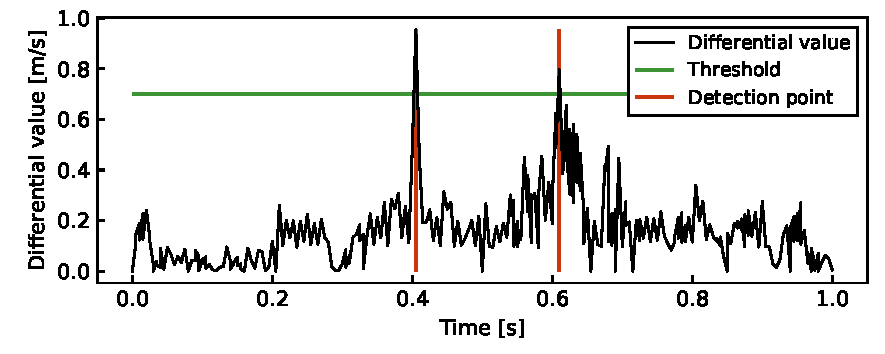
\includegraphics[width=11.5cm]{./fig/result_radar.pdf}
    \caption{路面までの距離の微分値の絶対値}
    \label{fig:result_radar}
\end{figure}

\section{考察}
 図\ref{fig:result_acc}に走行中の車両の加速度の推移を示す.システムが段差を検知した約50ms後に15m/s$^2$以上の加速度が車体に加わっていることがわかる.このことから,提案システムは車体に衝撃が加わる前に路面の段差をあらかじめ検出することができると結論づける.
\begin{figure}[H]
    \centering
    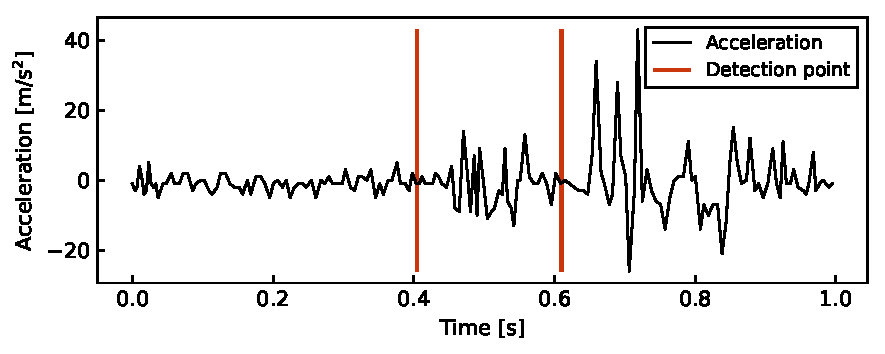
\includegraphics[width=11.5cm]{./fig/result_acc.pdf}
    \caption{車体に加わった上下方向の加速度}
    \label{fig:result_acc}
\end{figure}

\section{課題点}
しかし,提案したアルゴリズムにはいくつかの問題があると考えられる.考えうる課題点を以下に述べる.
\begin{enumerate}
    \item \textbf{発車時の振動による誤検知}\\
        このシステムではRADARから得られる距離の微分値(変化量)を基準に段差の有無を検出している.発車時のような車両の運動が急変する際にRADARが出力する距離の値に影響を及ぼす可能性がある.
    \item \textbf{旋回時での段差非検出}\\
        RADARは車両前面の1つのみで測定を行っている.カーブの先にある段差に関しては現状のシステムでは検出することは困難である.
    \item \textbf{閾値が実験的に導出されている}\\
        段差の検出に使用している微分絶対値の閾値は測定データを参考に手動でチューニングしたものであり,理論的に導出されたものでない.最終的に人が乗る車両のアクティブサスペンションの動作計画に活用することを考えると,その判定の責任を担保するためには理論的な閾値の導出が必要不可欠である.
\end{enumerate}
